
\documentclass[border=2]{standalone}
\usepackage{tikz}

\usetikzlibrary{arrows, arrows.meta, positioning}

\def\r{0.2}
\def\delta{0.05}
\def\yslant{0.5}
\def\xslant{0.0}
\def\gap{30}
\def\oPacity{0.8}

\tikzset{
    traj1/.style={ thick, dashed },
    traj2/.style={ very thin, dashed },
    traj3/.style={ thick },
    point/.style={ color=black, circle, scale=0.2, fill },
    label/.style={ scale=0.5, black, below = \r }
}

\newlength{\Lx}
\newlength{\Ly}

\newcommand{\drawFlock}[3]{
    \draw[fill=#3!50] (#1, #2) circle (\r);
    \node[point] at (#1 + 2*\delta, #2) {};
    \node[point] at (#1 - \delta,   #2 + 2*\delta) {};
    \node[point] at (#1 - \delta,   #2 - 2*\delta) {};
}

\newcommand{\drawLabel}[2]{
    \node[label] at (#1) {$#2$};
}

\newcommand{\drawTraj}[2]{
    \draw[traj1] (#1) -- (#2);
}

\newcommand{\drawTrajD}[2]{
    \draw[traj2] (#1) -- (#2);
}

\newcommand{\drawTrajF}[2]{
    \draw[traj3] (#1) -- (#2);
}

\begin{document}

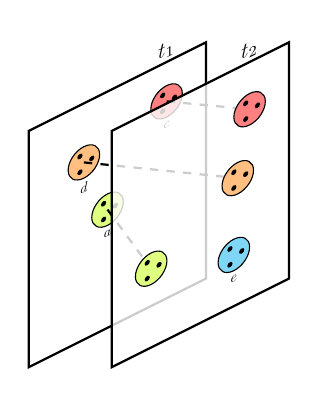
\begin{tikzpicture}
    %\draw[white] (0,0) rectangle (4.4,4.2);
    \def\t{0}
    \begin{scope}[
        xshift=\gap*\t,every node/.append style={        yslant=\yslant,xslant=\xslant},yslant=\yslant,xslant=\xslant]

        \node[scale=0.75, left=3mm] at (2.25,3.0) {$t_{1}$};
        \coordinate (A\t) at (1.00, 1.50);
        \coordinate (C\t) at (1.75, 2.50);
        \coordinate (D\t) at (0.70, 2.25);

        \drawTraj{A0}{A\t}
        \drawTrajF{C0}{C\t}
        \fill[white, thick, fill opacity=\oPacity] (0,0) rectangle (2.25,3.0);
        \draw[black, thick] (0,0) rectangle (2.25,3.0);

        \drawFlock{1.00}{1.50}{lime};
        \drawFlock{1.75}{2.50}{red};
        \drawFlock{0.70}{2.25}{orange};

        \drawLabel{A\t}{a};
        \drawLabel{C\t}{c};
        \drawLabel{D\t}{d};
    \end{scope}

    \def\t{1}
    \begin{scope}[
        xshift=\gap*\t,every node/.append style={        yslant=\yslant,xslant=\xslant},yslant=\yslant,xslant=\xslant]

        \node[scale=0.75, left=3mm] at (2.25,3.0) {$t_{2}$};
        \coordinate (A\t) at (0.50, 1.00);
        \coordinate (C\t) at (1.75, 2.40);
        \coordinate (D\t) at (1.60, 1.60);
        \coordinate (E\t) at (1.55, 0.65);

        \drawTraj{A0}{A\t}
        \drawTraj{C0}{C\t}
        \drawTraj{D0}{D\t}

        \fill[white, thick, fill opacity=\oPacity] (0,0) rectangle (2.25,3.0);
        \draw[black, thick] (0,0) rectangle (2.25,3.0);

        \drawFlock{0.50}{1.00}{lime};
        \drawFlock{1.55}{0.65}{cyan};
        \drawFlock{1.75}{2.40}{red};
        \drawFlock{1.60}{1.60}{orange};

        \drawLabel{E\t}{e};
    \end{scope}

\end{tikzpicture}

\end{document}
